\documentclass[1p]{elsarticle_modified}
%\bibliographystyle{elsarticle-num}

%\usepackage[colorlinks]{hyperref}
%\usepackage{abbrmath_seonhwa} %\Abb, \Ascr, \Acal ,\Abf, \Afrak
\usepackage{amsfonts}
\usepackage{amssymb}
\usepackage{amsmath}
\usepackage{amsthm}
\usepackage{scalefnt}
\usepackage{amsbsy}
\usepackage{kotex}
\usepackage{caption}
\usepackage{subfig}
\usepackage{color}
\usepackage{graphicx}
\usepackage{xcolor} %% white, black, red, green, blue, cyan, magenta, yellow
\usepackage{float}
\usepackage{setspace}
\usepackage{hyperref}

\usepackage{tikz}
\usetikzlibrary{arrows}

\usepackage{multirow}
\usepackage{array} % fixed length table
\usepackage{hhline}

%%%%%%%%%%%%%%%%%%%%%
\makeatletter
\renewcommand*\env@matrix[1][\arraystretch]{%
	\edef\arraystretch{#1}%
	\hskip -\arraycolsep
	\let\@ifnextchar\new@ifnextchar
	\array{*\c@MaxMatrixCols c}}
\makeatother %https://tex.stackexchange.com/questions/14071/how-can-i-increase-the-line-spacing-in-a-matrix
%%%%%%%%%%%%%%%

\usepackage[normalem]{ulem}

\newcommand{\msout}[1]{\ifmmode\text{\sout{\ensuremath{#1}}}\else\sout{#1}\fi}
%SOURCE: \msout is \stkout macro in https://tex.stackexchange.com/questions/20609/strikeout-in-math-mode

\newcommand{\cancel}[1]{
	\ifmmode
	{\color{red}\msout{#1}}
	\else
	{\color{red}\sout{#1}}
	\fi
}

\newcommand{\add}[1]{
	{\color{blue}\uwave{#1}}
}

\newcommand{\replace}[2]{
	\ifmmode
	{\color{red}\msout{#1}}{\color{blue}\uwave{#2}}
	\else
	{\color{red}\sout{#1}}{\color{blue}\uwave{#2}}
	\fi
}

\newcommand{\Sol}{\mathcal{S}} %segment
\newcommand{\D}{D} %diagram
\newcommand{\A}{\mathcal{A}} %arc


%%%%%%%%%%%%%%%%%%%%%%%%%%%%%5 test

\def\sl{\operatorname{\textup{SL}}(2,\Cbb)}
\def\psl{\operatorname{\textup{PSL}}(2,\Cbb)}
\def\quan{\mkern 1mu \triangleright \mkern 1mu}

\theoremstyle{definition}
\newtheorem{thm}{Theorem}[section]
\newtheorem{prop}[thm]{Proposition}
\newtheorem{lem}[thm]{Lemma}
\newtheorem{ques}[thm]{Question}
\newtheorem{cor}[thm]{Corollary}
\newtheorem{defn}[thm]{Definition}
\newtheorem{exam}[thm]{Example}
\newtheorem{rmk}[thm]{Remark}
\newtheorem{alg}[thm]{Algorithm}

\newcommand{\I}{\sqrt{-1}}
\begin{document}

%\begin{frontmatter}
%
%\title{Boundary parabolic representations of knots up to 8 crossings}
%
%%% Group authors per affiliation:
%\author{Yunhi Cho} 
%\address{Department of Mathematics, University of Seoul, Seoul, Korea}
%\ead{yhcho@uos.ac.kr}
%
%
%\author{Seonhwa Kim} %\fnref{s_kim}}
%\address{Center for Geometry and Physics, Institute for Basic Science, Pohang, 37673, Korea}
%\ead{ryeona17@ibs.re.kr}
%
%\author{Hyuk Kim}
%\address{Department of Mathematical Sciences, Seoul National University, Seoul 08826, Korea}
%\ead{hyukkim@snu.ac.kr}
%
%\author{Seokbeom Yoon}
%\address{Department of Mathematical Sciences, Seoul National University, Seoul, 08826,  Korea}
%\ead{sbyoon15@snu.ac.kr}
%
%\begin{abstract}
%We find all boundary parabolic representation of knots up to 8 crossings.
%
%\end{abstract}
%\begin{keyword}
%    \MSC[2010] 57M25 
%\end{keyword}
%
%\end{frontmatter}

%\linenumbers
%\tableofcontents
%
\newcommand\colored[1]{\textcolor{white}{\rule[-0.35ex]{0.8em}{1.4ex}}\kern-0.8em\color{red} #1}%
%\newcommand\colored[1]{\textcolor{white}{ #1}\kern-2.17ex	\textcolor{white}{ #1}\kern-1.81ex	\textcolor{white}{ #1}\kern-2.15ex\color{red}#1	}

{\Large $\underline{11n_{22}~(K11n_{22})}$}

\setlength{\tabcolsep}{10pt}
\renewcommand{\arraystretch}{1.6}
\vspace{1cm}\begin{tabular}{m{100pt}>{\centering\arraybackslash}m{274pt}}
\multirow{5}{120pt}{
	\centering
	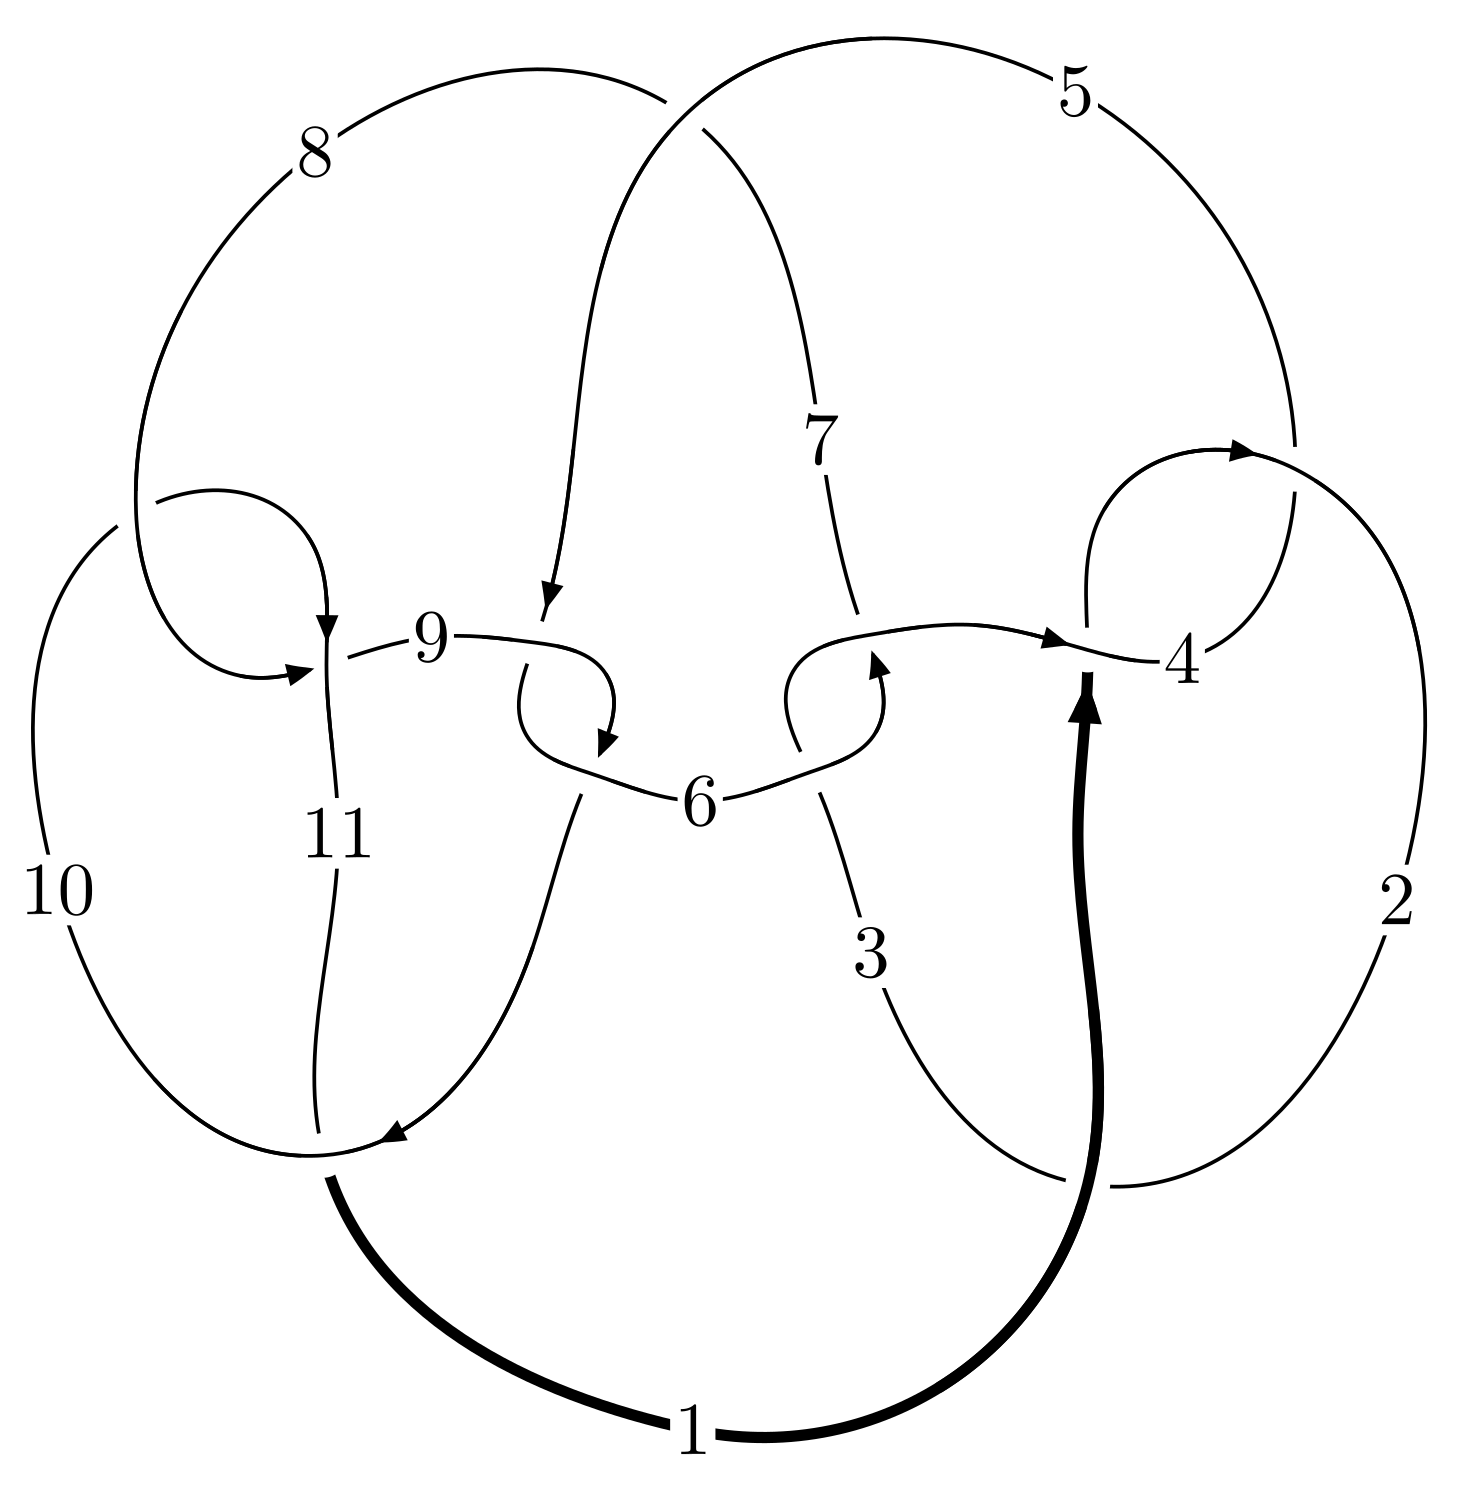
\includegraphics[width=112pt]{../../../GIT/diagram.site/Diagrams/png/638_11n_22.png}\\
\ \ \ A knot diagram\footnotemark}&
\allowdisplaybreaks
\textbf{Linearized knot diagam} \\
\cline{2-2}
 &
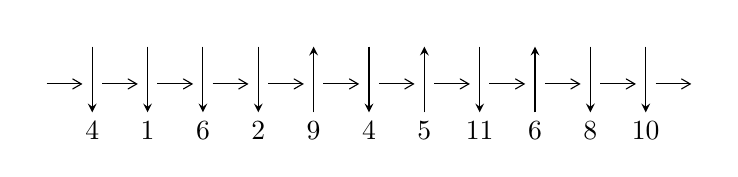
\begin{tikzpicture}[x=20pt, y=17pt]
	% nodes
	\node (C0) at (0, 0) {};
	\node (C1) at (1, 0) {};
	\node (C1U) at (1, +1) {};
	\node (C1D) at (1, -1) {4};

	\node (C2) at (2, 0) {};
	\node (C2U) at (2, +1) {};
	\node (C2D) at (2, -1) {1};

	\node (C3) at (3, 0) {};
	\node (C3U) at (3, +1) {};
	\node (C3D) at (3, -1) {6};

	\node (C4) at (4, 0) {};
	\node (C4U) at (4, +1) {};
	\node (C4D) at (4, -1) {2};

	\node (C5) at (5, 0) {};
	\node (C5U) at (5, +1) {};
	\node (C5D) at (5, -1) {9};

	\node (C6) at (6, 0) {};
	\node (C6U) at (6, +1) {};
	\node (C6D) at (6, -1) {4};

	\node (C7) at (7, 0) {};
	\node (C7U) at (7, +1) {};
	\node (C7D) at (7, -1) {5};

	\node (C8) at (8, 0) {};
	\node (C8U) at (8, +1) {};
	\node (C8D) at (8, -1) {11};

	\node (C9) at (9, 0) {};
	\node (C9U) at (9, +1) {};
	\node (C9D) at (9, -1) {6};

	\node (C10) at (10, 0) {};
	\node (C10U) at (10, +1) {};
	\node (C10D) at (10, -1) {8};

	\node (C11) at (11, 0) {};
	\node (C11U) at (11, +1) {};
	\node (C11D) at (11, -1) {10};
	\node (C12) at (12, 0) {};

	% arrows
	\draw[->,>={angle 60}]
	(C0) edge (C1) (C1) edge (C2) (C2) edge (C3) (C3) edge (C4) (C4) edge (C5) (C5) edge (C6) (C6) edge (C7) (C7) edge (C8) (C8) edge (C9) (C9) edge (C10) (C10) edge (C11) (C11) edge (C12) ;	\draw[->,>=stealth]
	(C1U) edge (C1D) (C2U) edge (C2D) (C3U) edge (C3D) (C4U) edge (C4D) (C5D) edge (C5U) (C6U) edge (C6D) (C7D) edge (C7U) (C8U) edge (C8D) (C9D) edge (C9U) (C10U) edge (C10D) (C11U) edge (C11D) ;
	\end{tikzpicture} \\
\hhline{~~} \\& 
\textbf{Solving Sequence} \\ \cline{2-2} 
 &
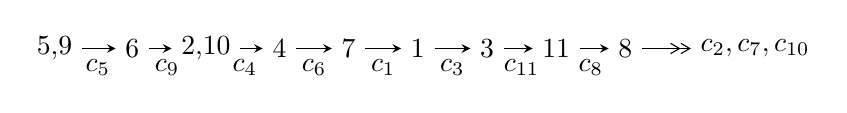
\begin{tikzpicture}[x=25pt, y=7pt]
	% node
	\node (A0) at (-1/8, 0) {5,9};
	\node (A1) at (1, 0) {6};
	\node (A2) at (33/16, 0) {2,10};
	\node (A3) at (25/8, 0) {4};
	\node (A4) at (33/8, 0) {7};
	\node (A5) at (41/8, 0) {1};
	\node (A6) at (49/8, 0) {3};
	\node (A7) at (57/8, 0) {11};
	\node (A8) at (65/8, 0) {8};
	\node (C1) at (1/2, -1) {$c_{5}$};
	\node (C2) at (3/2, -1) {$c_{9}$};
	\node (C3) at (21/8, -1) {$c_{4}$};
	\node (C4) at (29/8, -1) {$c_{6}$};
	\node (C5) at (37/8, -1) {$c_{1}$};
	\node (C6) at (45/8, -1) {$c_{3}$};
	\node (C7) at (53/8, -1) {$c_{11}$};
	\node (C8) at (61/8, -1) {$c_{8}$};
	\node (A9) at (10, 0) {$c_{2},c_{7},c_{10}$};

	% edge
	\draw[->,>=stealth]	
	(A0) edge (A1) (A1) edge (A2) (A2) edge (A3) (A3) edge (A4) (A4) edge (A5) (A5) edge (A6) (A6) edge (A7) (A7) edge (A8) ;
	\draw[->>,>={angle 60}]	
	(A8) edge (A9);
\end{tikzpicture} \\ 

\end{tabular} \\

\footnotetext{
The image of knot diagram is generated by the software ``\textbf{Draw programme}" developed by Andrew Bartholomew(\url{http://www.layer8.co.uk/maths/draw/index.htm\#Running-draw}), where we modified some parts for our purpose(\url{https://github.com/CATsTAILs/LinksPainter}).
}\phantom \\ \newline 
\centering \textbf{Ideals for irreducible components\footnotemark of $X_{\text{par}}$} 
 
\begin{align*}
I^u_{1}&=\langle 
1.10514\times10^{39} u^{35}+3.11173\times10^{39} u^{34}+\cdots+2.41739\times10^{40} b+4.96908\times10^{40},\\
\phantom{I^u_{1}}&\phantom{= \langle  }9.97702\times10^{39} u^{35}+3.04436\times10^{39} u^{34}+\cdots+4.83478\times10^{40} a+6.03959\times10^{39},\;u^{36}+2 u^{35}+\cdots-4 u+8\rangle \\
I^u_{2}&=\langle 
b+1,\;u^5-2 u^3+u^2+a+2 u,\;u^6- u^5- u^4+2 u^3- u+1\rangle \\
\\
I^v_{1}&=\langle 
a,\;- v^2+b-3 v+1,\;v^3+2 v^2-3 v+1\rangle \\
\end{align*}
\raggedright * 3 irreducible components of $\dim_{\mathbb{C}}=0$, with total 45 representations.\\
\footnotetext{All coefficients of polynomials are rational numbers. But the coefficients are sometimes approximated in decimal forms when there is not enough margin.}
\newpage
\renewcommand{\arraystretch}{1}
\centering \section*{I. $I^u_{1}= \langle 1.11\times10^{39} u^{35}+3.11\times10^{39} u^{34}+\cdots+2.42\times10^{40} b+4.97\times10^{40},\;9.98\times10^{39} u^{35}+3.04\times10^{39} u^{34}+\cdots+4.83\times10^{40} a+6.04\times10^{39},\;u^{36}+2 u^{35}+\cdots-4 u+8 \rangle$}
\flushleft \textbf{(i) Arc colorings}\\
\begin{tabular}{m{7pt} m{180pt} m{7pt} m{180pt} }
\flushright $a_{5}=$&$\begin{pmatrix}1\\0\end{pmatrix}$ \\
\flushright $a_{9}=$&$\begin{pmatrix}0\\u\end{pmatrix}$ \\
\flushright $a_{6}=$&$\begin{pmatrix}1\\- u^2\end{pmatrix}$ \\
\flushright $a_{2}=$&$\begin{pmatrix}-0.206359 u^{35}-0.0629680 u^{34}+\cdots+2.74530 u-0.124920\\-0.0457161 u^{35}-0.128723 u^{34}+\cdots+2.35374 u-2.05556\end{pmatrix}$ \\
\flushright $a_{10}=$&$\begin{pmatrix}u\\- u^3+u\end{pmatrix}$ \\
\flushright $a_{4}=$&$\begin{pmatrix}0.427443 u^{35}+0.372711 u^{34}+\cdots+0.384288 u+4.31112\\0.198044 u^{35}+0.422790 u^{34}+\cdots-10.2169 u+3.38570\end{pmatrix}$ \\
\flushright $a_{7}=$&$\begin{pmatrix}0.0303222 u^{35}+0.0626215 u^{34}+\cdots-2.77119 u-0.192221\\-0.188410 u^{35}-0.280513 u^{34}+\cdots+8.45275 u-2.80684\end{pmatrix}$ \\
\flushright $a_{1}=$&$\begin{pmatrix}0.0303222 u^{35}+0.0626215 u^{34}+\cdots-2.77119 u-0.192221\\0.119317 u^{35}+0.288516 u^{34}+\cdots-8.21808 u+2.82265\end{pmatrix}$ \\
\flushright $a_{3}=$&$\begin{pmatrix}1.17216 u^{35}+1.26150 u^{34}+\cdots-15.1808 u+11.5542\\-0.361331 u^{35}-0.145692 u^{34}+\cdots-1.85662 u-1.41937\end{pmatrix}$ \\
\flushright $a_{11}=$&$\begin{pmatrix}0.0556923 u^{35}+0.131200 u^{34}+\cdots-4.42903 u+0.594050\\0.223465 u^{35}+0.365609 u^{34}+\cdots-9.74431 u+3.75163\end{pmatrix}$ \\
\flushright $a_{8}=$&$\begin{pmatrix}-0.158088 u^{35}-0.217892 u^{34}+\cdots+5.68156 u-2.99906\\-0.188410 u^{35}-0.280513 u^{34}+\cdots+8.45275 u-2.80684\end{pmatrix}$\\ \flushright $a_{8}=$&$\begin{pmatrix}-0.158088 u^{35}-0.217892 u^{34}+\cdots+5.68156 u-2.99906\\-0.188410 u^{35}-0.280513 u^{34}+\cdots+8.45275 u-2.80684\end{pmatrix}$\\&\end{tabular}
\flushleft \textbf{(ii) Obstruction class $= -1$}\\~\\
\flushleft \textbf{(iii) Cusp Shapes $= 0.408352 u^{35}+0.642649 u^{34}+\cdots-18.9306 u-3.95860$}\\~\\
\newpage\renewcommand{\arraystretch}{1}
\flushleft \textbf{(iv) u-Polynomials at the component}\newline \\
\begin{tabular}{m{50pt}|m{274pt}}
Crossings & \hspace{64pt}u-Polynomials at each crossing \\
\hline $$\begin{aligned}c_{1},c_{4}\end{aligned}$$&$\begin{aligned}
&u^{36}-8 u^{35}+\cdots-6 u+1
\end{aligned}$\\
\hline $$\begin{aligned}c_{2}\end{aligned}$$&$\begin{aligned}
&u^{36}+8 u^{35}+\cdots+22 u+1
\end{aligned}$\\
\hline $$\begin{aligned}c_{3},c_{6}\end{aligned}$$&$\begin{aligned}
&u^{36}-2 u^{35}+\cdots-384 u^2-64
\end{aligned}$\\
\hline $$\begin{aligned}c_{5},c_{9}\end{aligned}$$&$\begin{aligned}
&u^{36}-2 u^{35}+\cdots+4 u+8
\end{aligned}$\\
\hline $$\begin{aligned}c_{7}\end{aligned}$$&$\begin{aligned}
&u^{36}+3 u^{35}+\cdots- u-1
\end{aligned}$\\
\hline $$\begin{aligned}c_{8},c_{10}\end{aligned}$$&$\begin{aligned}
&u^{36}-5 u^{35}+\cdots+18 u-1
\end{aligned}$\\
\hline $$\begin{aligned}c_{11}\end{aligned}$$&$\begin{aligned}
&u^{36}+15 u^{35}+\cdots+218 u+1
\end{aligned}$\\
\hline
\end{tabular}\\~\\
\newpage\renewcommand{\arraystretch}{1}
\flushleft \textbf{(v) Riley Polynomials at the component}\newline \\
\begin{tabular}{m{50pt}|m{274pt}}
Crossings & \hspace{64pt}Riley Polynomials at each crossing \\
\hline $$\begin{aligned}c_{1},c_{4}\end{aligned}$$&$\begin{aligned}
&y^{36}-8 y^{35}+\cdots-22 y+1
\end{aligned}$\\
\hline $$\begin{aligned}c_{2}\end{aligned}$$&$\begin{aligned}
&y^{36}+48 y^{35}+\cdots-22 y+1
\end{aligned}$\\
\hline $$\begin{aligned}c_{3},c_{6}\end{aligned}$$&$\begin{aligned}
&y^{36}+42 y^{35}+\cdots+49152 y+4096
\end{aligned}$\\
\hline $$\begin{aligned}c_{5},c_{9}\end{aligned}$$&$\begin{aligned}
&y^{36}-24 y^{35}+\cdots-1488 y+64
\end{aligned}$\\
\hline $$\begin{aligned}c_{7}\end{aligned}$$&$\begin{aligned}
&y^{36}-45 y^{35}+\cdots-5 y+1
\end{aligned}$\\
\hline $$\begin{aligned}c_{8},c_{10}\end{aligned}$$&$\begin{aligned}
&y^{36}-15 y^{35}+\cdots-218 y+1
\end{aligned}$\\
\hline $$\begin{aligned}c_{11}\end{aligned}$$&$\begin{aligned}
&y^{36}+17 y^{35}+\cdots-43646 y+1
\end{aligned}$\\
\hline
\end{tabular}\\~\\
\newpage\flushleft \textbf{(vi) Complex Volumes and Cusp Shapes}
$$\begin{array}{c|c|c}  
\text{Solutions to }I^u_{1}& \I (\text{vol} + \sqrt{-1}CS) & \text{Cusp shape}\\
 \hline 
\begin{aligned}
u &= -0.876781 + 0.467791 I \\
a &= \phantom{-}0.771077 - 0.499574 I \\
b &= \phantom{-}0.458159 + 0.388133 I\end{aligned}
 & \phantom{-}1.44120 - 1.68807 I & \phantom{-}1.23787 + 2.98942 I \\ \hline\begin{aligned}
u &= -0.876781 - 0.467791 I \\
a &= \phantom{-}0.771077 + 0.499574 I \\
b &= \phantom{-}0.458159 - 0.388133 I\end{aligned}
 & \phantom{-}1.44120 + 1.68807 I & \phantom{-}1.23787 - 2.98942 I \\ \hline\begin{aligned}
u &= \phantom{-}0.562796 + 0.711448 I \\
a &= \phantom{-}0.798144 + 0.463491 I \\
b &= \phantom{-}0.364530 + 0.110500 I\end{aligned}
 & -2.24151 - 1.11055 I & -4.16932 + 0.85691 I \\ \hline\begin{aligned}
u &= \phantom{-}0.562796 - 0.711448 I \\
a &= \phantom{-}0.798144 - 0.463491 I \\
b &= \phantom{-}0.364530 - 0.110500 I\end{aligned}
 & -2.24151 + 1.11055 I & -4.16932 - 0.85691 I \\ \hline\begin{aligned}
u &= -1.149490 + 0.105847 I \\
a &= -0.69354 - 2.02575 I \\
b &= \phantom{-}0.973276 + 0.948498 I\end{aligned}
 & \phantom{-}3.87982 - 3.49544 I & -3.17810 + 2.67745 I \\ \hline\begin{aligned}
u &= -1.149490 - 0.105847 I \\
a &= -0.69354 + 2.02575 I \\
b &= \phantom{-}0.973276 - 0.948498 I\end{aligned}
 & \phantom{-}3.87982 + 3.49544 I & -3.17810 - 2.67745 I \\ \hline\begin{aligned}
u &= \phantom{-}1.151290 + 0.136717 I \\
a &= -0.050534 + 0.984743 I \\
b &= -1.156680 - 0.402174 I\end{aligned}
 & \phantom{-}0.196716 + 1.191220 I & -3.75367 - 2.76129 I \\ \hline\begin{aligned}
u &= \phantom{-}1.151290 - 0.136717 I \\
a &= -0.050534 - 0.984743 I \\
b &= -1.156680 + 0.402174 I\end{aligned}
 & \phantom{-}0.196716 - 1.191220 I & -3.75367 + 2.76129 I \\ \hline\begin{aligned}
u &= \phantom{-}1.012080 + 0.596945 I \\
a &= \phantom{-}0.812755 + 0.396273 I \\
b &= \phantom{-}0.666828 - 0.220770 I\end{aligned}
 & -0.90609 + 6.15586 I & -1.06826 - 8.23147 I \\ \hline\begin{aligned}
u &= \phantom{-}1.012080 - 0.596945 I \\
a &= \phantom{-}0.812755 - 0.396273 I \\
b &= \phantom{-}0.666828 + 0.220770 I\end{aligned}
 & -0.90609 - 6.15586 I & -1.06826 + 8.23147 I\\
 \hline 
 \end{array}$$\newpage$$\begin{array}{c|c|c}  
\text{Solutions to }I^u_{1}& \I (\text{vol} + \sqrt{-1}CS) & \text{Cusp shape}\\
 \hline 
\begin{aligned}
u &= \phantom{-}0.132013 + 0.796085 I \\
a &= \phantom{-}0.530905 + 0.123801 I \\
b &= -0.363392 - 0.400261 I\end{aligned}
 & -1.17315 - 1.43837 I & -4.87286 + 4.95965 I \\ \hline\begin{aligned}
u &= \phantom{-}0.132013 - 0.796085 I \\
a &= \phantom{-}0.530905 - 0.123801 I \\
b &= -0.363392 + 0.400261 I\end{aligned}
 & -1.17315 + 1.43837 I & -4.87286 - 4.95965 I \\ \hline\begin{aligned}
u &= -1.188780 + 0.305866 I \\
a &= -0.477194 + 1.088200 I \\
b &= -1.293690 - 0.259633 I\end{aligned}
 & -0.19217 - 3.89522 I & -3.75583 + 3.33691 I \\ \hline\begin{aligned}
u &= -1.188780 - 0.305866 I \\
a &= -0.477194 - 1.088200 I \\
b &= -1.293690 + 0.259633 I\end{aligned}
 & -0.19217 + 3.89522 I & -3.75583 - 3.33691 I \\ \hline\begin{aligned}
u &= -0.114291 + 1.235990 I \\
a &= \phantom{-}0.468464 - 0.379839 I \\
b &= \phantom{-}0.919988 + 1.004770 I\end{aligned}
 & \phantom{-}5.76584 - 0.88624 I & -3.08966 - 0.19737 I \\ \hline\begin{aligned}
u &= -0.114291 - 1.235990 I \\
a &= \phantom{-}0.468464 + 0.379839 I \\
b &= \phantom{-}0.919988 - 1.004770 I\end{aligned}
 & \phantom{-}5.76584 + 0.88624 I & -3.08966 + 0.19737 I \\ \hline\begin{aligned}
u &= -0.299008 + 1.238570 I \\
a &= \phantom{-}0.478366 + 0.338536 I \\
b &= \phantom{-}1.040320 - 0.944822 I\end{aligned}
 & \phantom{-}5.37775 + 6.26456 I & -3.90154 - 4.74503 I \\ \hline\begin{aligned}
u &= -0.299008 - 1.238570 I \\
a &= \phantom{-}0.478366 - 0.338536 I \\
b &= \phantom{-}1.040320 + 0.944822 I\end{aligned}
 & \phantom{-}5.37775 - 6.26456 I & -3.90154 + 4.74503 I \\ \hline\begin{aligned}
u &= -1.282480 + 0.078351 I \\
a &= \phantom{-}0.406471 + 1.116480 I \\
b &= -0.272152 - 0.810511 I\end{aligned}
 & \phantom{-}3.60869 - 0.40430 I & -0.180320 + 0.512361 I \\ \hline\begin{aligned}
u &= -1.282480 - 0.078351 I \\
a &= \phantom{-}0.406471 - 1.116480 I \\
b &= -0.272152 + 0.810511 I\end{aligned}
 & \phantom{-}3.60869 + 0.40430 I & -0.180320 - 0.512361 I\\
 \hline 
 \end{array}$$\newpage$$\begin{array}{c|c|c}  
\text{Solutions to }I^u_{1}& \I (\text{vol} + \sqrt{-1}CS) & \text{Cusp shape}\\
 \hline 
\begin{aligned}
u &= \phantom{-}1.300550 + 0.426752 I \\
a &= \phantom{-}0.110638 - 1.292420 I \\
b &= -0.510437 + 0.832243 I\end{aligned}
 & \phantom{-}2.60051 + 6.07581 I & -2.58564 - 6.03076 I \\ \hline\begin{aligned}
u &= \phantom{-}1.300550 - 0.426752 I \\
a &= \phantom{-}0.110638 + 1.292420 I \\
b &= -0.510437 - 0.832243 I\end{aligned}
 & \phantom{-}2.60051 - 6.07581 I & -2.58564 + 6.03076 I \\ \hline\begin{aligned}
u &= -0.607835 + 0.068419 I \\
a &= \phantom{-}0.588549 + 0.355335 I \\
b &= \phantom{-}0.895986 - 0.665316 I\end{aligned}
 & \phantom{-}1.96162 + 2.57896 I & \phantom{-}2.96196 - 0.32171 I \\ \hline\begin{aligned}
u &= -0.607835 - 0.068419 I \\
a &= \phantom{-}0.588549 - 0.355335 I \\
b &= \phantom{-}0.895986 + 0.665316 I\end{aligned}
 & \phantom{-}1.96162 - 2.57896 I & \phantom{-}2.96196 + 0.32171 I \\ \hline\begin{aligned}
u &= -0.203337 + 0.520719 I \\
a &= -4.57730 + 1.89887 I \\
b &= -1.060050 + 0.082275 I\end{aligned}
 & -3.21515 + 0.53565 I & -7.7422 + 12.1700 I \\ \hline\begin{aligned}
u &= -0.203337 - 0.520719 I \\
a &= -4.57730 - 1.89887 I \\
b &= -1.060050 - 0.082275 I\end{aligned}
 & -3.21515 - 0.53565 I & -7.7422 - 12.1700 I \\ \hline\begin{aligned}
u &= \phantom{-}0.529202\phantom{ +0.000000I} \\
a &= \phantom{-}4.14663\phantom{ +0.000000I} \\
b &= -0.467103\phantom{ +0.000000I}\end{aligned}
 & -2.39731\phantom{ +0.000000I} & \phantom{-}2.58440\phantom{ +0.000000I} \\ \hline\begin{aligned}
u &= \phantom{-}1.45234 + 0.47903 I \\
a &= \phantom{-}0.18492 + 1.55929 I \\
b &= \phantom{-}1.12508 - 0.97464 I\end{aligned}
 & \phantom{-}10.93880 + 6.87915 I & \phantom{-0.000000 } 0. - 3.18853 I \\ \hline\begin{aligned}
u &= \phantom{-}1.45234 - 0.47903 I \\
a &= \phantom{-}0.18492 - 1.55929 I \\
b &= \phantom{-}1.12508 + 0.97464 I\end{aligned}
 & \phantom{-}10.93880 - 6.87915 I & \phantom{-0.000000 -}0. + 3.18853 I \\ \hline\begin{aligned}
u &= -1.36361 + 0.70201 I \\
a &= \phantom{-}0.52721 - 1.55915 I \\
b &= \phantom{-}1.17133 + 0.91175 I\end{aligned}
 & \phantom{-}8.7659 - 13.1890 I & -5.00000 + 7.32457 I\\
 \hline 
 \end{array}$$\newpage$$\begin{array}{c|c|c}  
\text{Solutions to }I^u_{1}& \I (\text{vol} + \sqrt{-1}CS) & \text{Cusp shape}\\
 \hline 
\begin{aligned}
u &= -1.36361 - 0.70201 I \\
a &= \phantom{-}0.52721 + 1.55915 I \\
b &= \phantom{-}1.17133 - 0.91175 I\end{aligned}
 & \phantom{-}8.7659 + 13.1890 I & -5.00000 - 7.32457 I \\ \hline\begin{aligned}
u &= \phantom{-}1.51813 + 0.32802 I \\
a &= -0.632543 - 0.937060 I \\
b &= \phantom{-}0.89682 + 1.12852 I\end{aligned}
 & \phantom{-}11.70850 - 0.74205 I & \phantom{-0.000000 } 0 \\ \hline\begin{aligned}
u &= \phantom{-}1.51813 - 0.32802 I \\
a &= -0.632543 + 0.937060 I \\
b &= \phantom{-}0.89682 - 1.12852 I\end{aligned}
 & \phantom{-}11.70850 + 0.74205 I & \phantom{-0.000000 } 0 \\ \hline\begin{aligned}
u &= -1.43939 + 0.60179 I \\
a &= -0.705793 + 0.628179 I \\
b &= \phantom{-}0.790568 - 1.152680 I\end{aligned}
 & \phantom{-}10.03080 - 5.72886 I & -5.00000 + 3.03607 I \\ \hline\begin{aligned}
u &= -1.43939 - 0.60179 I \\
a &= -0.705793 - 0.628179 I \\
b &= \phantom{-}0.790568 + 1.152680 I\end{aligned}
 & \phantom{-}10.03080 + 5.72886 I & -5.00000 - 3.03607 I \\ \hline\begin{aligned}
u &= \phantom{-}0.262401\phantom{ +0.000000I} \\
a &= \phantom{-}1.77219\phantom{ +0.000000I} \\
b &= -0.825866\phantom{ +0.000000I}\end{aligned}
 & -1.19842\phantom{ +0.000000I} & -8.63080\phantom{ +0.000000I}\\
 \hline 
 \end{array}$$\newpage\newpage\renewcommand{\arraystretch}{1}
\centering \section*{II. $I^u_{2}= \langle b+1,\;u^5-2 u^3+u^2+a+2 u,\;u^6- u^5- u^4+2 u^3- u+1 \rangle$}
\flushleft \textbf{(i) Arc colorings}\\
\begin{tabular}{m{7pt} m{180pt} m{7pt} m{180pt} }
\flushright $a_{5}=$&$\begin{pmatrix}1\\0\end{pmatrix}$ \\
\flushright $a_{9}=$&$\begin{pmatrix}0\\u\end{pmatrix}$ \\
\flushright $a_{6}=$&$\begin{pmatrix}1\\- u^2\end{pmatrix}$ \\
\flushright $a_{2}=$&$\begin{pmatrix}- u^5+2 u^3- u^2-2 u\\-1\end{pmatrix}$ \\
\flushright $a_{10}=$&$\begin{pmatrix}u\\- u^3+u\end{pmatrix}$ \\
\flushright $a_{4}=$&$\begin{pmatrix}- u^5+2 u^3- u^2-2 u+1\\-1\end{pmatrix}$ \\
\flushright $a_{7}=$&$\begin{pmatrix}1\\- u^2\end{pmatrix}$ \\
\flushright $a_{1}=$&$\begin{pmatrix}-1\\0\end{pmatrix}$ \\
\flushright $a_{3}=$&$\begin{pmatrix}- u^5+2 u^3- u^2-2 u+1\\-1\end{pmatrix}$ \\
\flushright $a_{11}=$&$\begin{pmatrix}- u^4+u^2-1\\u^5- u^4-2 u^3+u^2+u-1\end{pmatrix}$ \\
\flushright $a_{8}=$&$\begin{pmatrix}- u^2+1\\- u^2\end{pmatrix}$\\ \flushright $a_{8}=$&$\begin{pmatrix}- u^2+1\\- u^2\end{pmatrix}$\\&\end{tabular}
\flushleft \textbf{(ii) Obstruction class $= 1$}\\~\\
\flushleft \textbf{(iii) Cusp Shapes $= u^5-5 u^4- u^3+7 u^2-4 u-12$}\\~\\
\newpage\renewcommand{\arraystretch}{1}
\flushleft \textbf{(iv) u-Polynomials at the component}\newline \\
\begin{tabular}{m{50pt}|m{274pt}}
Crossings & \hspace{64pt}u-Polynomials at each crossing \\
\hline $$\begin{aligned}c_{1}\end{aligned}$$&$\begin{aligned}
&(u-1)^6
\end{aligned}$\\
\hline $$\begin{aligned}c_{2},c_{4}\end{aligned}$$&$\begin{aligned}
&(u+1)^6
\end{aligned}$\\
\hline $$\begin{aligned}c_{3},c_{6}\end{aligned}$$&$\begin{aligned}
&u^6
\end{aligned}$\\
\hline $$\begin{aligned}c_{5},c_{10}\end{aligned}$$&$\begin{aligned}
&u^6- u^5- u^4+2 u^3- u+1
\end{aligned}$\\
\hline $$\begin{aligned}c_{7}\end{aligned}$$&$\begin{aligned}
&u^6-3 u^5+5 u^4-4 u^3+2 u^2- u+1
\end{aligned}$\\
\hline $$\begin{aligned}c_{8},c_{9}\end{aligned}$$&$\begin{aligned}
&u^6+u^5- u^4-2 u^3+u+1
\end{aligned}$\\
\hline $$\begin{aligned}c_{11}\end{aligned}$$&$\begin{aligned}
&u^6+3 u^5+5 u^4+4 u^3+2 u^2+u+1
\end{aligned}$\\
\hline
\end{tabular}\\~\\
\newpage\renewcommand{\arraystretch}{1}
\flushleft \textbf{(v) Riley Polynomials at the component}\newline \\
\begin{tabular}{m{50pt}|m{274pt}}
Crossings & \hspace{64pt}Riley Polynomials at each crossing \\
\hline $$\begin{aligned}c_{1},c_{2},c_{4}\end{aligned}$$&$\begin{aligned}
&(y-1)^6
\end{aligned}$\\
\hline $$\begin{aligned}c_{3},c_{6}\end{aligned}$$&$\begin{aligned}
&y^6
\end{aligned}$\\
\hline $$\begin{aligned}c_{5},c_{8},c_{9}\\c_{10}\end{aligned}$$&$\begin{aligned}
&y^6-3 y^5+5 y^4-4 y^3+2 y^2- y+1
\end{aligned}$\\
\hline $$\begin{aligned}c_{7},c_{11}\end{aligned}$$&$\begin{aligned}
&y^6+y^5+5 y^4+6 y^2+3 y+1
\end{aligned}$\\
\hline
\end{tabular}\\~\\
\newpage\flushleft \textbf{(vi) Complex Volumes and Cusp Shapes}
$$\begin{array}{c|c|c}  
\text{Solutions to }I^u_{2}& \I (\text{vol} + \sqrt{-1}CS) & \text{Cusp shape}\\
 \hline 
\begin{aligned}
u &= -1.002190 + 0.295542 I \\
a &= -0.230593 + 0.497010 I \\
b &= -1.00000\phantom{ +0.000000I}\end{aligned}
 & \phantom{-}0.245672 - 0.924305 I & -3.44826 + 0.47256 I \\ \hline\begin{aligned}
u &= -1.002190 - 0.295542 I \\
a &= -0.230593 - 0.497010 I \\
b &= -1.00000\phantom{ +0.000000I}\end{aligned}
 & \phantom{-}0.245672 + 0.924305 I & -3.44826 - 0.47256 I \\ \hline\begin{aligned}
u &= \phantom{-}0.428243 + 0.664531 I \\
a &= -1.66103 - 1.45708 I \\
b &= -1.00000\phantom{ +0.000000I}\end{aligned}
 & -3.53554 - 0.92430 I & -13.66012 + 2.42665 I \\ \hline\begin{aligned}
u &= \phantom{-}0.428243 - 0.664531 I \\
a &= -1.66103 + 1.45708 I \\
b &= -1.00000\phantom{ +0.000000I}\end{aligned}
 & -3.53554 + 0.92430 I & -13.66012 - 2.42665 I \\ \hline\begin{aligned}
u &= \phantom{-}1.073950 + 0.558752 I \\
a &= -0.608378 - 0.558752 I \\
b &= -1.00000\phantom{ +0.000000I}\end{aligned}
 & -1.64493 + 5.69302 I & -8.89162 - 3.92918 I \\ \hline\begin{aligned}
u &= \phantom{-}1.073950 - 0.558752 I \\
a &= -0.608378 + 0.558752 I \\
b &= -1.00000\phantom{ +0.000000I}\end{aligned}
 & -1.64493 - 5.69302 I & -8.89162 + 3.92918 I\\
 \hline 
 \end{array}$$\newpage\newpage\renewcommand{\arraystretch}{1}
\centering \section*{III. $I^v_{1}= \langle a,\;- v^2+b-3 v+1,\;v^3+2 v^2-3 v+1 \rangle$}
\flushleft \textbf{(i) Arc colorings}\\
\begin{tabular}{m{7pt} m{180pt} m{7pt} m{180pt} }
\flushright $a_{5}=$&$\begin{pmatrix}1\\0\end{pmatrix}$ \\
\flushright $a_{9}=$&$\begin{pmatrix}v\\0\end{pmatrix}$ \\
\flushright $a_{6}=$&$\begin{pmatrix}1\\0\end{pmatrix}$ \\
\flushright $a_{2}=$&$\begin{pmatrix}0\\v^2+3 v-1\end{pmatrix}$ \\
\flushright $a_{10}=$&$\begin{pmatrix}v\\0\end{pmatrix}$ \\
\flushright $a_{4}=$&$\begin{pmatrix}1\\-2 v^2-5 v+3\end{pmatrix}$ \\
\flushright $a_{7}=$&$\begin{pmatrix}-2 v^2-5 v+4\\v^2+2 v-3\end{pmatrix}$ \\
\flushright $a_{1}=$&$\begin{pmatrix}v^2+3 v-1\\- v^2-2 v+3\end{pmatrix}$ \\
\flushright $a_{3}=$&$\begin{pmatrix}-2 v^2-5 v+4\\-2 v^2-5 v+3\end{pmatrix}$ \\
\flushright $a_{11}=$&$\begin{pmatrix}v^2+4 v-1\\- v^2-2 v+3\end{pmatrix}$ \\
\flushright $a_{8}=$&$\begin{pmatrix}- v^2-3 v+1\\v^2+2 v-3\end{pmatrix}$\\ \flushright $a_{8}=$&$\begin{pmatrix}- v^2-3 v+1\\v^2+2 v-3\end{pmatrix}$\\&\end{tabular}
\flushleft \textbf{(ii) Obstruction class $= 1$}\\~\\
\flushleft \textbf{(iii) Cusp Shapes $= 6 v^2+19 v-21$}\\~\\
\newpage\renewcommand{\arraystretch}{1}
\flushleft \textbf{(iv) u-Polynomials at the component}\newline \\
\begin{tabular}{m{50pt}|m{274pt}}
Crossings & \hspace{64pt}u-Polynomials at each crossing \\
\hline $$\begin{aligned}c_{1}\end{aligned}$$&$\begin{aligned}
&u^3+u^2-1
\end{aligned}$\\
\hline $$\begin{aligned}c_{2},c_{6}\end{aligned}$$&$\begin{aligned}
&u^3+u^2+2 u+1
\end{aligned}$\\
\hline $$\begin{aligned}c_{3}\end{aligned}$$&$\begin{aligned}
&u^3- u^2+2 u-1
\end{aligned}$\\
\hline $$\begin{aligned}c_{4}\end{aligned}$$&$\begin{aligned}
&u^3- u^2+1
\end{aligned}$\\
\hline $$\begin{aligned}c_{5},c_{9}\end{aligned}$$&$\begin{aligned}
&u^3
\end{aligned}$\\
\hline $$\begin{aligned}c_{7}\end{aligned}$$&$\begin{aligned}
&u^3-3 u^2+2 u+1
\end{aligned}$\\
\hline $$\begin{aligned}c_{8}\end{aligned}$$&$\begin{aligned}
&(u-1)^3
\end{aligned}$\\
\hline $$\begin{aligned}c_{10},c_{11}\end{aligned}$$&$\begin{aligned}
&(u+1)^3
\end{aligned}$\\
\hline
\end{tabular}\\~\\
\newpage\renewcommand{\arraystretch}{1}
\flushleft \textbf{(v) Riley Polynomials at the component}\newline \\
\begin{tabular}{m{50pt}|m{274pt}}
Crossings & \hspace{64pt}Riley Polynomials at each crossing \\
\hline $$\begin{aligned}c_{1},c_{4}\end{aligned}$$&$\begin{aligned}
&y^3- y^2+2 y-1
\end{aligned}$\\
\hline $$\begin{aligned}c_{2},c_{3},c_{6}\end{aligned}$$&$\begin{aligned}
&y^3+3 y^2+2 y-1
\end{aligned}$\\
\hline $$\begin{aligned}c_{5},c_{9}\end{aligned}$$&$\begin{aligned}
&y^3
\end{aligned}$\\
\hline $$\begin{aligned}c_{7}\end{aligned}$$&$\begin{aligned}
&y^3-5 y^2+10 y-1
\end{aligned}$\\
\hline $$\begin{aligned}c_{8},c_{10},c_{11}\end{aligned}$$&$\begin{aligned}
&(y-1)^3
\end{aligned}$\\
\hline
\end{tabular}\\~\\
\newpage\flushleft \textbf{(vi) Complex Volumes and Cusp Shapes}
$$\begin{array}{c|c|c}  
\text{Solutions to }I^v_{1}& \I (\text{vol} + \sqrt{-1}CS) & \text{Cusp shape}\\
 \hline 
\begin{aligned}
v &= \phantom{-}0.539798 + 0.182582 I \\
a &= \phantom{-0.000000 } 0 \\
b &= \phantom{-}0.877439 + 0.744862 I\end{aligned}
 & \phantom{-}1.37919 - 2.82812 I & -9.19557 + 4.65175 I \\ \hline\begin{aligned}
v &= \phantom{-}0.539798 - 0.182582 I \\
a &= \phantom{-0.000000 } 0 \\
b &= \phantom{-}0.877439 - 0.744862 I\end{aligned}
 & \phantom{-}1.37919 + 2.82812 I & -9.19557 - 4.65175 I \\ \hline\begin{aligned}
v &= -3.07960\phantom{ +0.000000I} \\
a &= \phantom{-0.000000 } 0 \\
b &= -0.754878\phantom{ +0.000000I}\end{aligned}
 & -2.75839\phantom{ +0.000000I} & -22.6090\phantom{ +0.000000I}\\
 \hline 
 \end{array}$$\newpage
\newpage\renewcommand{\arraystretch}{1}
\centering \section*{ IV. u-Polynomials}
\begin{tabular}{m{50pt}|m{274pt}}
Crossings & \hspace{64pt}u-Polynomials at each crossing \\
\hline $$\begin{aligned}c_{1}\end{aligned}$$&$\begin{aligned}
&((u-1)^6)(u^3+u^2-1)(u^{36}-8 u^{35}+\cdots-6 u+1)
\end{aligned}$\\
\hline $$\begin{aligned}c_{2}\end{aligned}$$&$\begin{aligned}
&((u+1)^6)(u^3+u^2+2 u+1)(u^{36}+8 u^{35}+\cdots+22 u+1)
\end{aligned}$\\
\hline $$\begin{aligned}c_{3}\end{aligned}$$&$\begin{aligned}
&u^6(u^3- u^2+2 u-1)(u^{36}-2 u^{35}+\cdots-384 u^{2}-64)
\end{aligned}$\\
\hline $$\begin{aligned}c_{4}\end{aligned}$$&$\begin{aligned}
&((u+1)^6)(u^3- u^2+1)(u^{36}-8 u^{35}+\cdots-6 u+1)
\end{aligned}$\\
\hline $$\begin{aligned}c_{5}\end{aligned}$$&$\begin{aligned}
&u^3(u^6- u^5+\cdots- u+1)(u^{36}-2 u^{35}+\cdots+4 u+8)
\end{aligned}$\\
\hline $$\begin{aligned}c_{6}\end{aligned}$$&$\begin{aligned}
&u^6(u^3+u^2+2 u+1)(u^{36}-2 u^{35}+\cdots-384 u^{2}-64)
\end{aligned}$\\
\hline $$\begin{aligned}c_{7}\end{aligned}$$&$\begin{aligned}
&(u^3-3 u^2+2 u+1)(u^6-3 u^5+5 u^4-4 u^3+2 u^2- u+1)\\
&\cdot(u^{36}+3 u^{35}+\cdots- u-1)
\end{aligned}$\\
\hline $$\begin{aligned}c_{8}\end{aligned}$$&$\begin{aligned}
&((u-1)^3)(u^6+u^5+\cdots+u+1)(u^{36}-5 u^{35}+\cdots+18 u-1)
\end{aligned}$\\
\hline $$\begin{aligned}c_{9}\end{aligned}$$&$\begin{aligned}
&u^3(u^6+u^5+\cdots+u+1)(u^{36}-2 u^{35}+\cdots+4 u+8)
\end{aligned}$\\
\hline $$\begin{aligned}c_{10}\end{aligned}$$&$\begin{aligned}
&((u+1)^3)(u^6- u^5+\cdots- u+1)(u^{36}-5 u^{35}+\cdots+18 u-1)
\end{aligned}$\\
\hline $$\begin{aligned}c_{11}\end{aligned}$$&$\begin{aligned}
&(u+1)^3(u^6+3 u^5+5 u^4+4 u^3+2 u^2+u+1)\\
&\cdot(u^{36}+15 u^{35}+\cdots+218 u+1)
\end{aligned}$\\
\hline
\end{tabular}\newpage\renewcommand{\arraystretch}{1}
\centering \section*{ V. Riley Polynomials}
\begin{tabular}{m{50pt}|m{274pt}}
Crossings & \hspace{64pt}Riley Polynomials at each crossing \\
\hline $$\begin{aligned}c_{1},c_{4}\end{aligned}$$&$\begin{aligned}
&((y-1)^6)(y^3- y^2+2 y-1)(y^{36}-8 y^{35}+\cdots-22 y+1)
\end{aligned}$\\
\hline $$\begin{aligned}c_{2}\end{aligned}$$&$\begin{aligned}
&((y-1)^6)(y^3+3 y^2+2 y-1)(y^{36}+48 y^{35}+\cdots-22 y+1)
\end{aligned}$\\
\hline $$\begin{aligned}c_{3},c_{6}\end{aligned}$$&$\begin{aligned}
&y^6(y^3+3 y^2+2 y-1)(y^{36}+42 y^{35}+\cdots+49152 y+4096)
\end{aligned}$\\
\hline $$\begin{aligned}c_{5},c_{9}\end{aligned}$$&$\begin{aligned}
&y^3(y^6-3 y^5+\cdots- y+1)(y^{36}-24 y^{35}+\cdots-1488 y+64)
\end{aligned}$\\
\hline $$\begin{aligned}c_{7}\end{aligned}$$&$\begin{aligned}
&(y^3-5 y^2+10 y-1)(y^6+y^5+5 y^4+6 y^2+3 y+1)\\
&\cdot(y^{36}-45 y^{35}+\cdots-5 y+1)
\end{aligned}$\\
\hline $$\begin{aligned}c_{8},c_{10}\end{aligned}$$&$\begin{aligned}
&(y-1)^3(y^6-3 y^5+5 y^4-4 y^3+2 y^2- y+1)\\
&\cdot(y^{36}-15 y^{35}+\cdots-218 y+1)
\end{aligned}$\\
\hline $$\begin{aligned}c_{11}\end{aligned}$$&$\begin{aligned}
&((y-1)^3)(y^6+y^5+\cdots+3 y+1)(y^{36}+17 y^{35}+\cdots-43646 y+1)
\end{aligned}$\\
\hline
\end{tabular}
\vskip 2pc
\end{document}